% \section{Experiments}\label{sec:experiments}

% \subsection{Experimental Setup}
% \shortparagraph{Dataset.} 
% To ensure a fair comparison across different rollout sampling strategies, we follow the Minimal-RL recipe~\citep{xiong2025minimalist} and train all models on the Numina-Math dataset~\citep{numina_math_7b}, which contains 860k math prompts paired with ground-truth answers. 
% %

% \shortparagraph{Models.}
% We conduct experiments with both Qwen-2.5-Math-1.5B~\citep{yang2024qwen2} and Llama-3.2-1B-Instruct~\citep{dubey2024llama}\footnote{We also experimented with the Llama-3.2-1B Base~\citep{dubey2024llama}; however, consistent with the observation of \citet{wang2025octothinker}, training base models with RL without proper mid-training (domain-specific fine-tuning) is challenging, yielding limited performance gains for all methods. We leave a more thorough investigation of this direction for future work.} to ensure generality, following the advice promoting rigorous RLVR evaluation~\citep{shao2025spurious, wu2025reasoning}. We additionally experiment with  Qwen-2.5-Math-7B model to see how well our methods generalize with model size scaling. 
% %

% \textbf{Baselines.}
% We evaluate \alg against standard fixed-temperature sampling with temperatures $\tau \in \{0.6, 1.0, 1.2\}$. 
% %
% % \zz{Should we mention these fixed-temp sampling are combined with GRPO, DAPO and GPG?}
% These values are chosen based on recommendations from prior work to establish strong baselines~\citep{renze-2024-effect, guo2025deepseek, hou2025t1}.
% %
% For a fair and controlled comparison, we disable two features for all methods: 
% (1) dynamic sampling~\citep{yu2025dapo}, to ensure all prompts are used during training;
% and (2) rollout length penalties, to avoid biasing the sampling process. 
% %
% As discussed in \cref{sec: method}, these techniques are orthogonal to our contribution and we leave further investigation about these to future work.
% %
% % \ych{Shall we demonstrate a case that with all techniques in place, using standard training recipe like DAPO, how well our model could be?}


% \shortparagraph{Implementation details.}
% Most experiments are conducted within DAPO~\citep{yu2025dapo} algorithms. To test whether \alg can apply to various RL algorithm, we additionally test \alg in GRPO~\citep{shao2024deepseekmath} and EntropyMech~\citep{cui2025entropy} using the same training and evaluation setup. 
% %
% More training details and hyperparameter setups are illustrated in \cref{app: minimal_rl_training_details}. 
% %
% Unless otherwise specified, we set $\tau_{\max}=1.2$ and $d=25$ as the default configuration for \alg.
% %
% We empirically find that for larger model with stronger generative capability, using an overly small $\tau_{\text{small}}$ would trigger the model to generate seemingly correct but wrong answers over the held-out validation set. 
% %
% For 1B models, we use $\tau_{\min}=0.1$ and we use $\tau_{\text{small}}=0.8$. All hyperparameters are tuned based on a prior study over held-out datasets. 
%
% \zz{might need to re-phrase since we only mention 1B models in this section, but I guess we are still waiting for llama 8B}


\section{Experiments}\label{sec:experiments}
\begin{figure}[t]
\centering
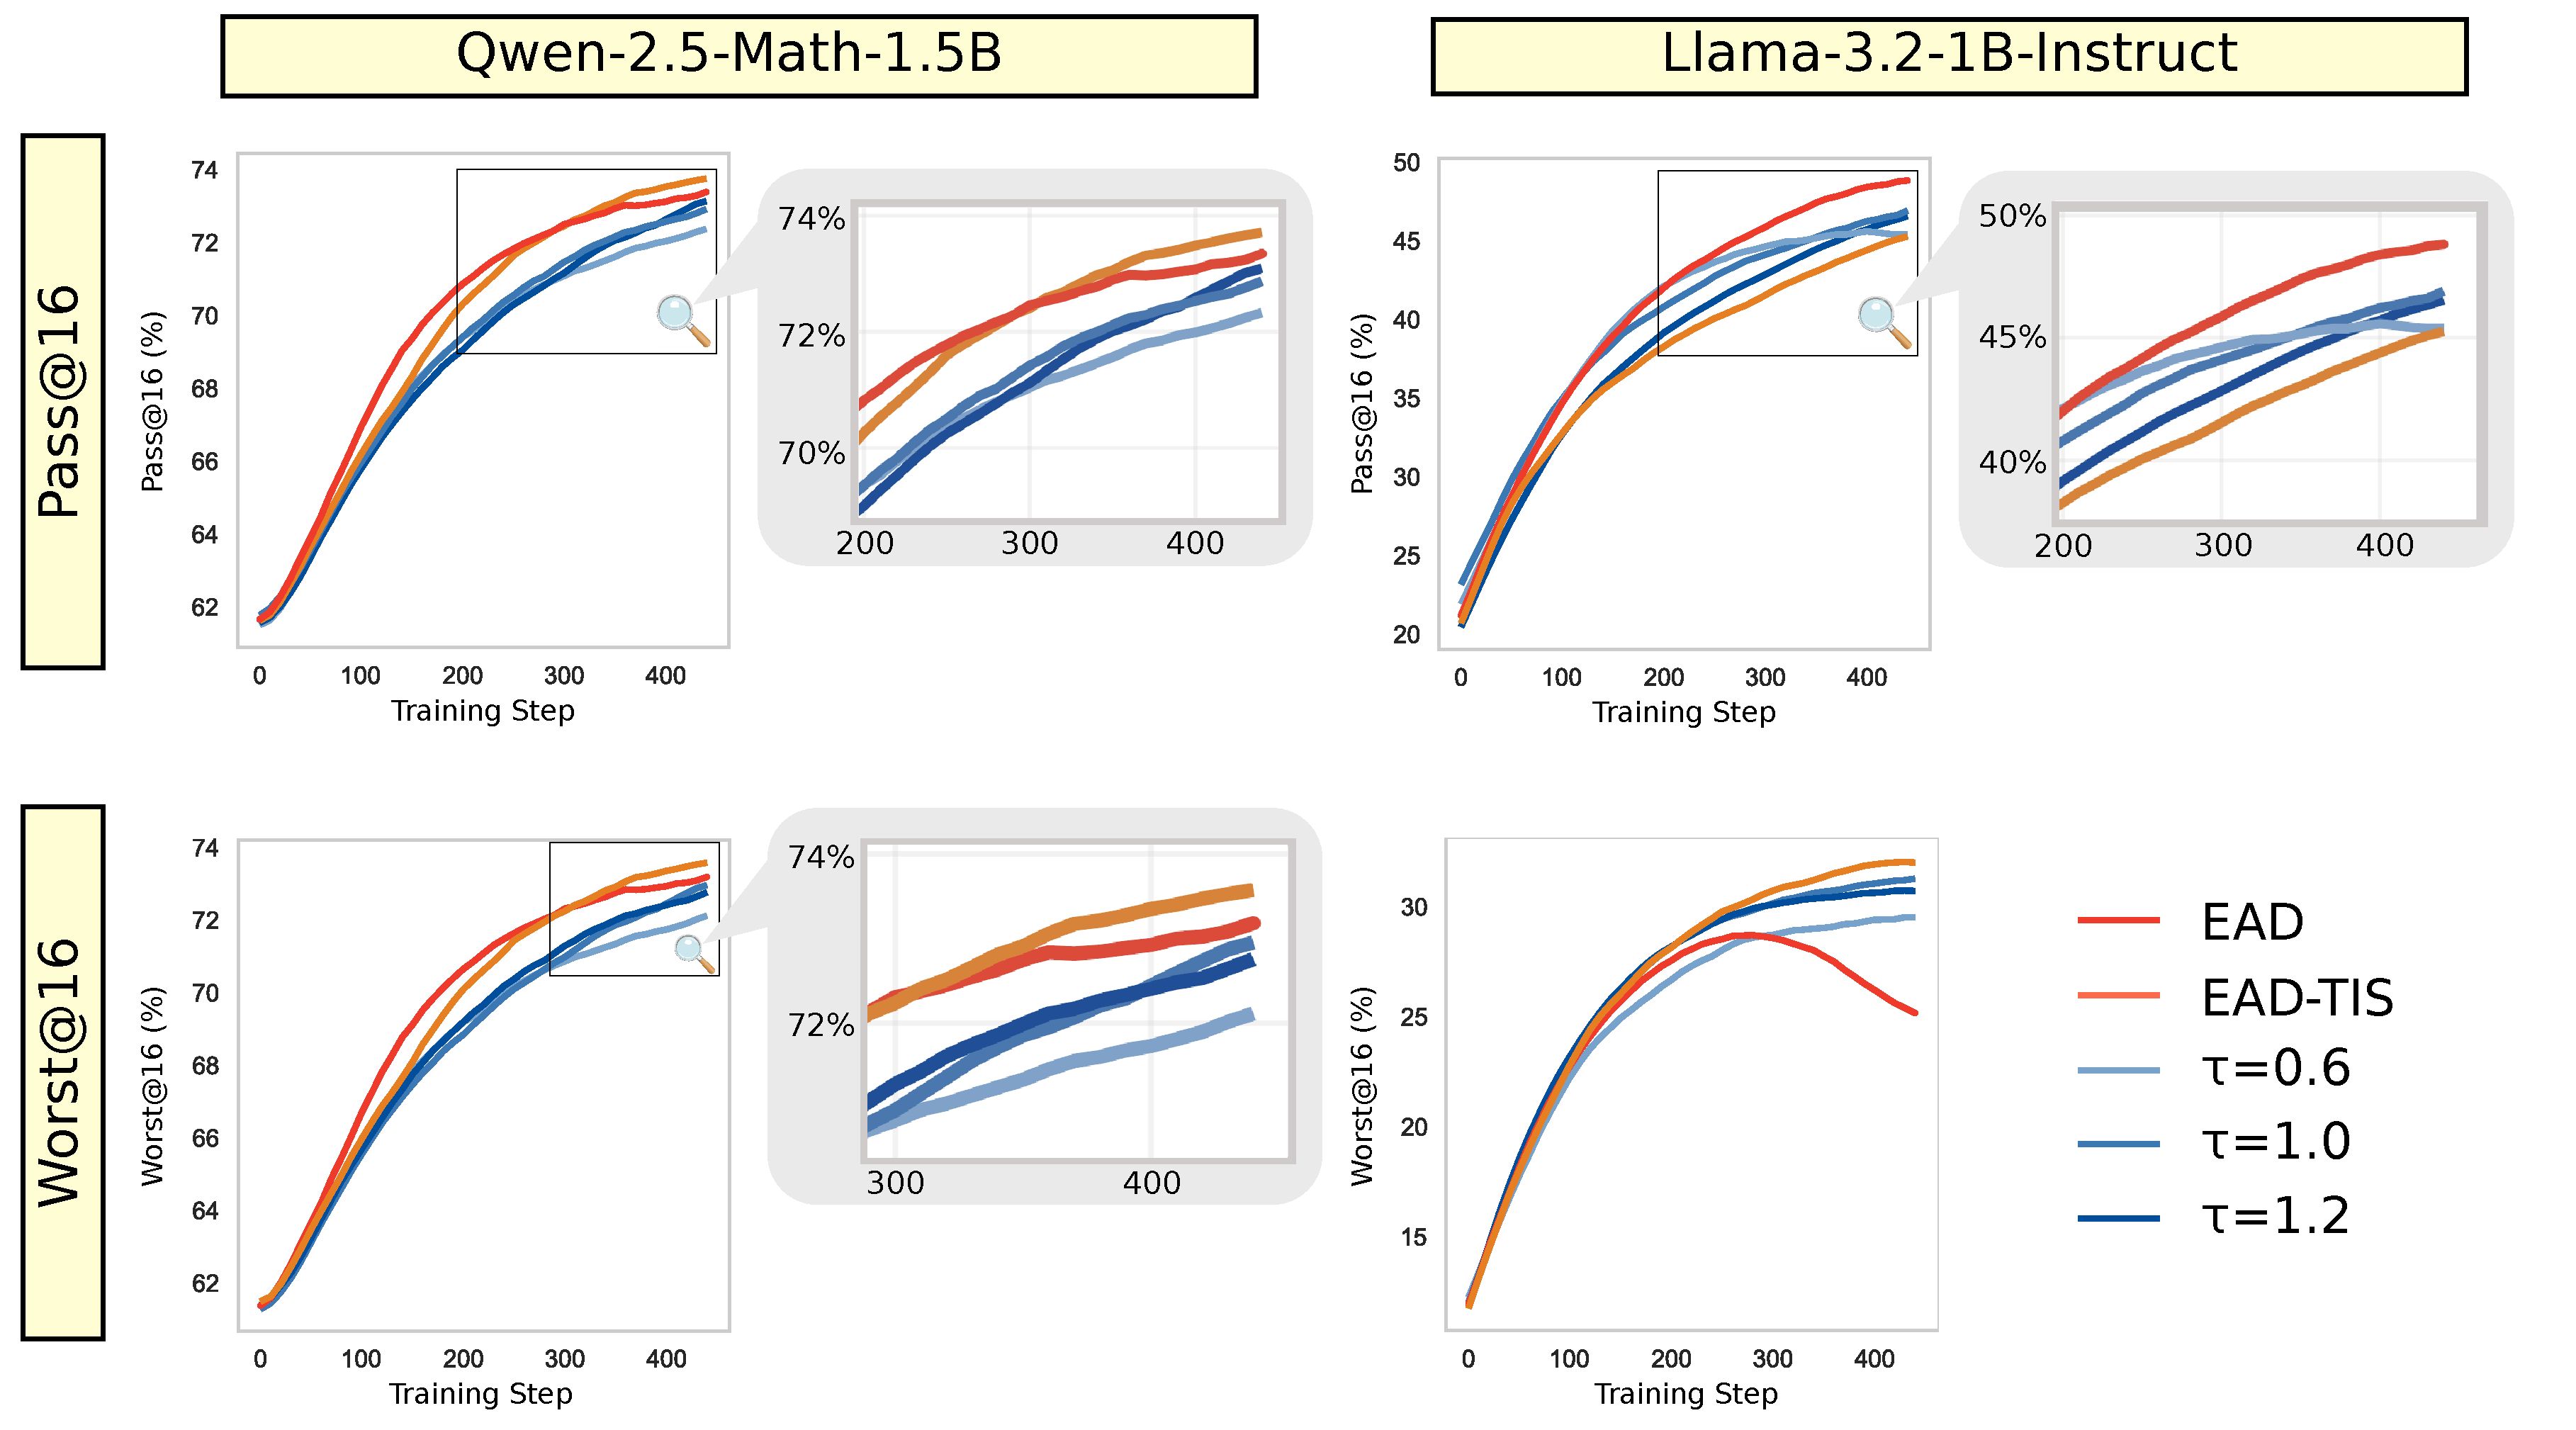
\includegraphics[width=0.7\linewidth]{figures/best-and-worst-at-16.pdf}
\vspace{-10pt}
\caption{
Pass@16 and Worst@16 evaluation in RL training. 
While \alg improves exploration of high-quality samples (even the worst outperform temperature sampling), the gain diminishes over time; TIS can supplement to correct bias and sustain training.
}
\label{fig: main_bench_best_worst_at_16}
\vspace{-13pt}
\end{figure}
%
% \begin{figure}[!ht]
%     \centering
%     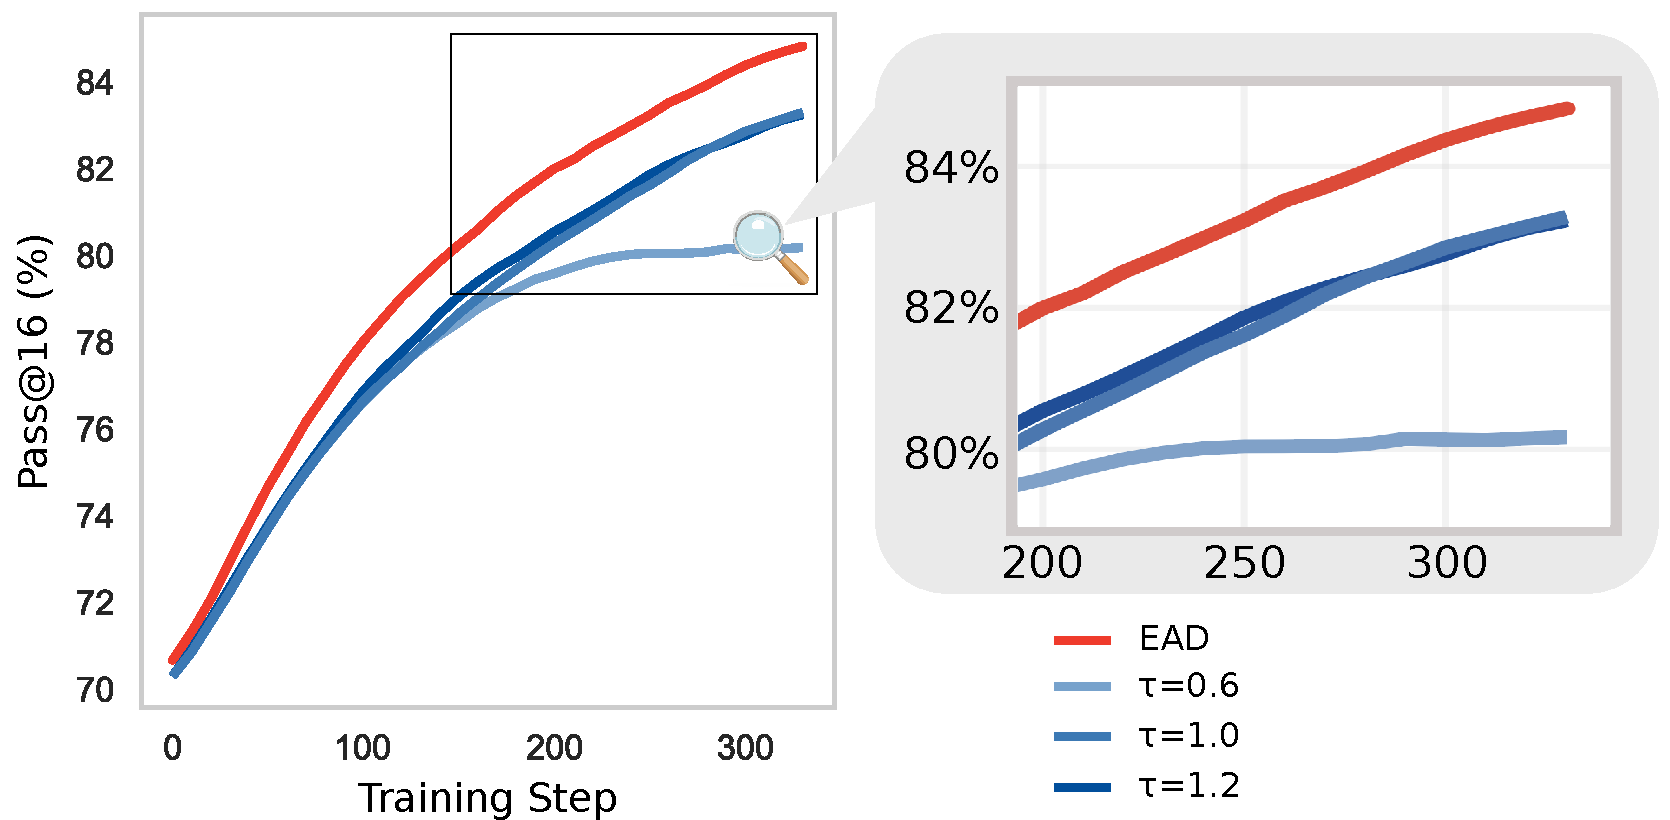
\includegraphics[width=0.6\linewidth]{figures/best_at_16_Qwen2.5-Math-7B.pdf}
%     \caption{
%     % Qwen-2.5-7B
%     Pass@16 performance on Qwen-2.5-Math-7B. 
%     %
%     \alg enables better exploration than fixed-temperature sampling, yielding sustained gains in Pass@16 throughout training.
%     %
%     }
%     \label{fig: best_at_16_qwen2.5_7b}
%     \vspace{-20pt}
% \end{figure}
%

\subsection{Experimental Setup}
\label{sec: experiment_setup}
\shortparagraph{Models, Data, and Training Frameworks.}
To ensure a rigorous and controlled comparison, we follow the Minimal-RL recipe~\citep{xiong2025minimalist},\footnote{More training details and hyperparameter setups are illustrated in \cref{app: minimal_rl_training_details}. } training all models on the Numina-Math dataset~\citep{numina_math_7b}, which contains 860k math prompts. We experiment with both Qwen-2.5-Math-1.5B~\citep{yang2024qwen2} and Llama-3.2-1B-Instruct~\citep{dubey2024llama}.\footnote{We also experimented with the Llama-3.2-1B base model. However, consistent with \citet{wang2025octothinker}, we found that applying RL to base models without intermediate domain-specific fine-tuning yields limited gains across all methods. We defer a deeper investigation to future work.} We also include the larger Qwen-2.5-Math-7B model to evaluate how our approach scales. While our primary experiments are conducted within the DAPO framework~\citep{yu2025dapo}, we demonstrate broader applicability by additionally integrating \alg with GRPO~\citep{shao2024deepseekmath} and EntropyMech~\citep{cui2025entropy}.

\shortparagraph{Baselines and Controlled Comparison.}
We evaluate \alg against fixed-temperature sampling, with temperatures $\tau \in \{0.6, 1.0, 1.2\}$ as recommended by prior work~\citep{renze-2024-effect, guo2025deepseek, hou2025t1}. For a fair comparison focused specifically on the sampling strategy, we disable two orthogonal techniques for all methods: (1) dynamic data sampling~\citep{yu2025dapo}, to maintain a consistent training set, and (2) rollout length penalties, to avoid confounding the reward signal with length-based biases.

\shortparagraph{Hyperparameters and Tuning.}
Unless otherwise stated, we use a default configuration of $\tau_{\max}=1.2$, $d_0=25$, $\alpha = 5$, and $d_{\max}=40000$ for \alg. 
%
For $\tau_{\min}$, we observed optimal values varied by model capability.
%
For the 1B and 1.5B models, we set $\tau_{\min}=0.1$. 
%
For the more capable 7B model, we used a higher value of $\tau_{\min}=0.8$, as stronger models already have sharper next-token distributions; a moderately high floor temperature prevents overconfident, near-greedy decoding that produces plausible but incorrect answers. The key benefit of \alg still holds: early tokens are sampled at a higher temperature than later ones, preserving the ``explore early, exploit late'' dynamic even within this narrower range.
%
All hyperparameters, including the learning rates for both \alg and the fixed-temperature baselines, were carefully tuned based on a prior study over held-out datasets to ensure a fair comparison. We also provide a detailed ablation study on the sensitivity of these hyperparameters in \cref{sec:ablation_study} to demonstrate the robustness of \alg.
%

% \subsection{\algname Improves RLVR Performance}
\subsection{\alg Improves RLVR Training}

% \begin{figure}[!ht]
%     \centering
%     \includegraphics[width=0.6\linewidth]{}
%     \caption{
%     % Qwen-2.5-7B
%     Pass@16 performance on Qwen-2.5-Math-7B. 
%     %
%     \alg enables better exploration than fixed-temperature sampling, yielding sustained gains in Pass@16 throughout training.
%     %
%     }
%     \label{fig: best_at_16_qwen2.5_7b}
%     \vspace{-20pt}
% \end{figure}
% \begin{figure}[!ht]
%     \centering
%     \includegraphics[width=0.6\linewidth]{}
%     \caption{
%     % Qwen-2.5-7B
%     Pass@16 performance on Qwen-2.5-Math-7B. 
%     %
%     \alg enables better exploration than fixed-temperature sampling, yielding sustained gains in Pass@16 throughout training.
%     %
%     }
%     \label{fig: best_at_16_qwen2.5_7b}
%     \vspace{-20pt}
% \end{figure}
% \begin{figure}[!ht]
%     \centering
%     \includegraphics[width=0.6\linewidth]{}
%     \caption{
%     % Qwen-2.5-7B
%     Pass@16 performance on Qwen-2.5-Math-7B. 
%     %
%     \alg enables better exploration than fixed-temperature sampling, yielding sustained gains in Pass@16 throughout training.
%     %
%     }
%     \label{fig: best_at_16_qwen2.5_7b}
%     \vspace{-20pt}
% \end{figure}
% \begin{figure}[!ht]
%     \centering
%     \includegraphics[width=0.6\linewidth]{}
%     \caption{
%     % Qwen-2.5-7B
%     Pass@16 performance on Qwen-2.5-Math-7B. 
%     %
%     \alg enables better exploration than fixed-temperature sampling, yielding sustained gains in Pass@16 throughout training.
%     %
%     }
%     \label{fig: best_at_16_qwen2.5_7b}
%     \vspace{-20pt}
% \end{figure}
\shortparagraph{\alg Improves RL Exploration and Training Efficiency.}
As shown in \cref{fig: main_bench_best_worst_at_16}, \alg significantly improves training efficiency. 
%
For Pass@16 accuracy, 
% both \alg (w/o TIS) and \alg (w/ TIS) 
\alg (w/o TIS) consistently outperforms the baselines on the Llama and Qwen models (\alg (w/ TIS) also outperforms on the Llama model), demonstrating more effective exploration. \begin{wrapfigure}{r}{0.35\textwidth}
    \centering
    % \vspace{-5pt} % Adjust to align the top of the figure with the text line
    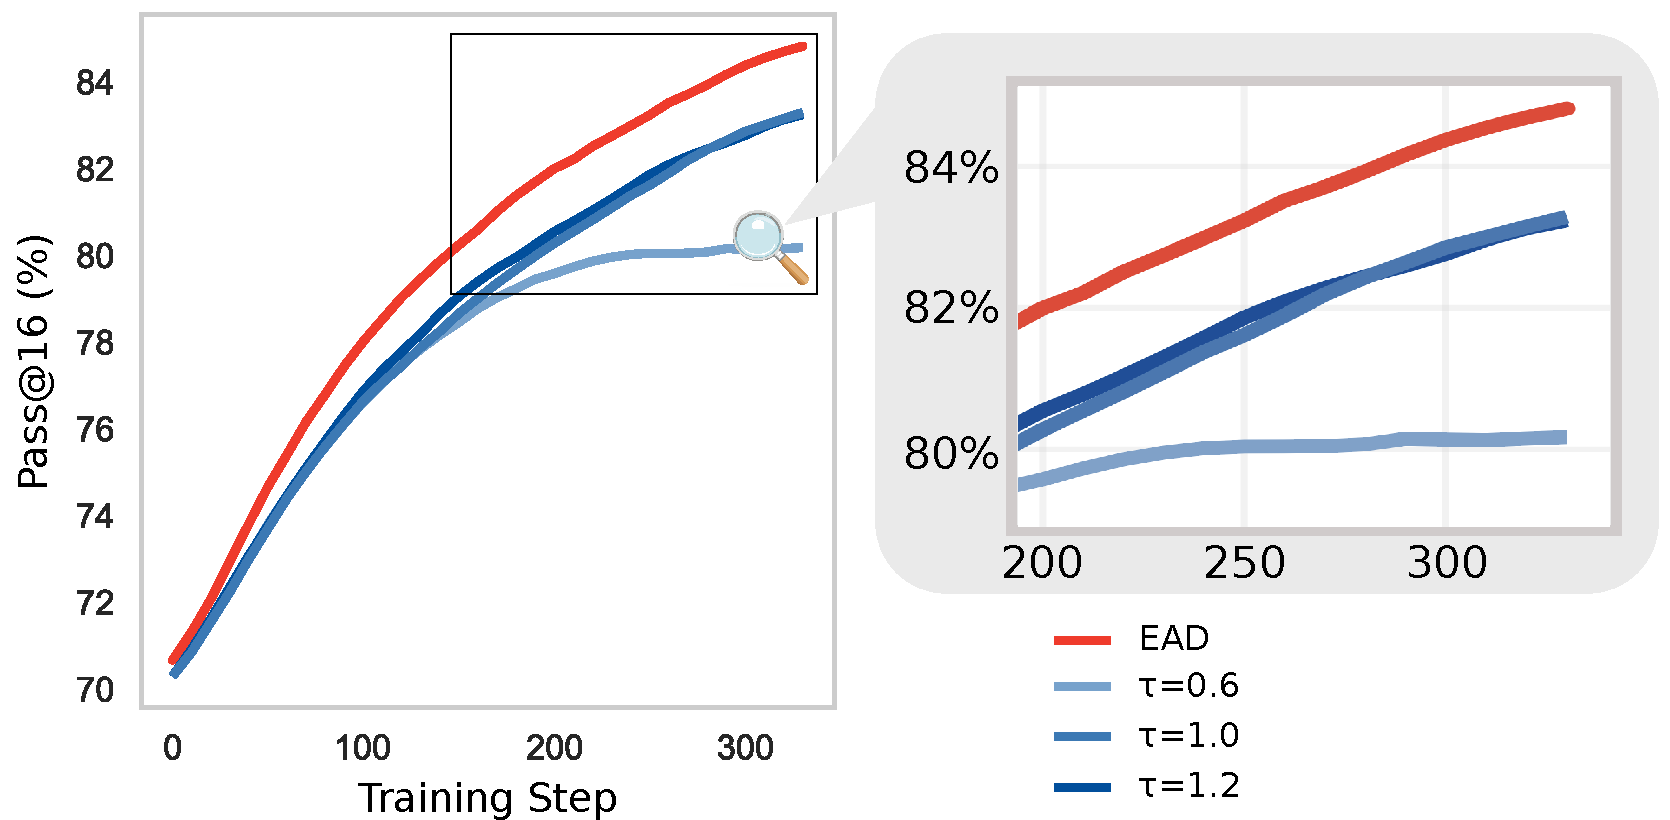
\includegraphics[width=\linewidth]{figures/best_at_16_Qwen2.5-Math-7B.pdf}
    \caption{
        Pass@16 on Qwen-2.5-Math-7B. \alg enables better exploration than fixed-temperature sampling, yielding sustained gains in Pass@16 throughout training.
    }
    \label{fig: best_at_16_qwen2.5_7b}
    \vspace{-18pt} % Adjust to manage spacing with the text below
\end{wrapfigure}
%
Under the stricter Worst@16 metric, the inclusion of TIS becomes essential for maintaining stable performance gains, highlighting its importance for correcting the off-policy training dynamic introduced by \alg. 
%
Through bootstrapping evaluation as in~\citet{hochlehnert2025sober}, the standard deviation of both Pass@16 performance and Worst@16 are way below 0.01 and thus all comparisons here are significant.
%
%
%
To verify that our method generalizes, we evaluated it on the larger Qwen-2.5-Math-7B model. The results, presented in \cref{fig: best_at_16_qwen2.5_7b}, confirm that the performance gains from \alg remain significant. This demonstrates that our approach is effective not only on smaller models but also scales successfully.
%

\begin{wrapfigure}{r}{0.55\textwidth}
    \centering
    \vspace{-15pt} % Pulls the figure up to align with the paragraph top
    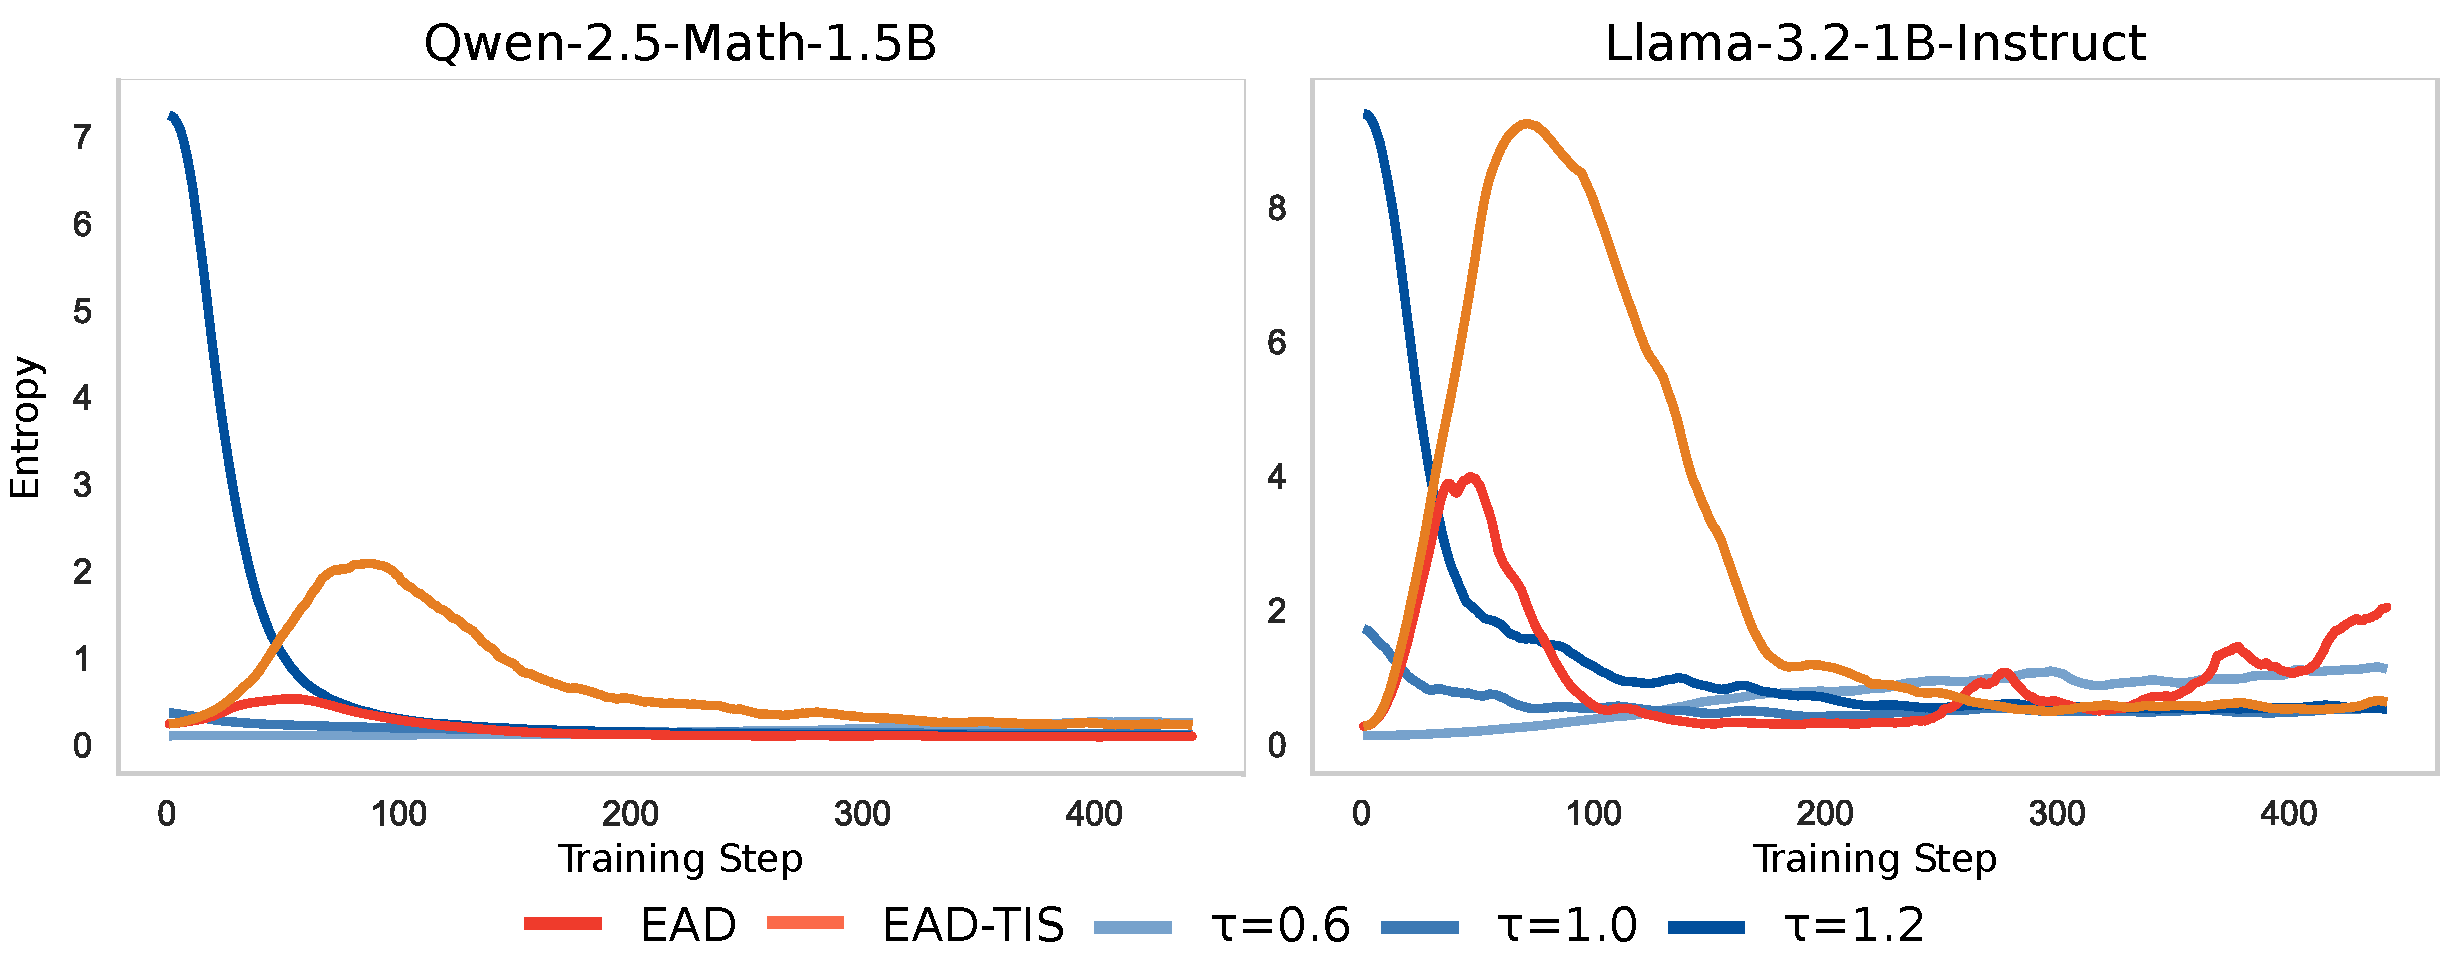
\includegraphics[width=\linewidth]{figures/entropy.pdf}
    \vspace{-15pt}
    \caption{
        Entropy dynamics. Fixed temperature sampling leads to a sharp decrease, while EAD maintains exploration to escape local minima.
    }
    \label{fig: main_bench_entropy}
    \vspace{-10pt} % Reduces white space below the figure
\end{wrapfigure}
\shortparagraph{\alg Mitigates Entropy Collapse.}
One major problem in RLVR training is entropy collapse~\citep{cui2025entropy}, which shrinks the exploration space and constrains improvement during the ``plateau stage''~\citep{deng2025trial}.
%
We plot the entropy dynamic in \cref{fig: main_bench_entropy}, where we can see that the entropy dynamic for \alg-empowered methods is not monotonically decreasing from the beginning. 
%
Instead, it tries to gradually transition out from local optimum~\citep{kirkpatrick1983optimization, bertsimas1993simulated} in a natural, continuous way without any external intervention, such as introducing tree search in rollout sampling~\citep{li2025treepo}.
%

\shortparagraph{Sample efficiency of \alg.}
Increasing the number of rollouts is a common but computationally expensive strategy to enhance exploration~\citep{hou2025t1}. 
%
We test the sample efficiency of \alg by varying the number of rollouts, adjusting the learning rate accordingly as suggested by prior work~\citep{chen2025pass}. 
%
As shown in \cref{fig: main_bench_rollout_scaling}, while more rollouts can further improve performance, \alg achieves strong results with just 4 or 8 rollouts. 
%
For instance, the optimal configurations are $n=8$ with a learning rate of $10^{-6}$ for Llama-3.2-1B-Instruct and $2\times10^{-6}$ for Qwen-2.5-Math-1.5B. 
%
This highlights the sample efficiency of our approach, offering a way to reduce the computational cost of the rollout phase.
%

% \shortparagraph{Disentangling Length and Quality.}
% A natural consequence of improved exploration is that \alg can induce slightly longer reasoning chains (see \cref{app: increased_length} for a detailed comparison of response lengths). However, several lines of evidence strongly suggest that the gains are primarily driven by the intra-sequence temperature schedule rather than simply from generating longer outputs: (1) the reverse annealing schedule (\cref{fig: reverse_annealing}), which also injects randomness and can produce longer responses, fails to match even standard temperature sampling; and (2) \alg improves inference-time Majority@$N$ on off-the-shelf models (\cref{fig: inference_time_scaling}), where no RL-induced length increase is present.
% %
% To assess whether \alg's advantage persists with extensive exploration, we compare it against baselines using a larger set of 16 rollouts. 
% %
% \cref{fig: rollout_modelwise_compare} shows that although the relative performance gain diminishes, \alg still outperforms fixed-temperature baselines by a clear margin.
% %


\subsection{\alg is Compatible with Various RL Algorithms}\begin{wrapfigure}{r}{0.5\textwidth}
    \centering
    \vspace{-15pt} % Adjust to align the top of the image with the text
    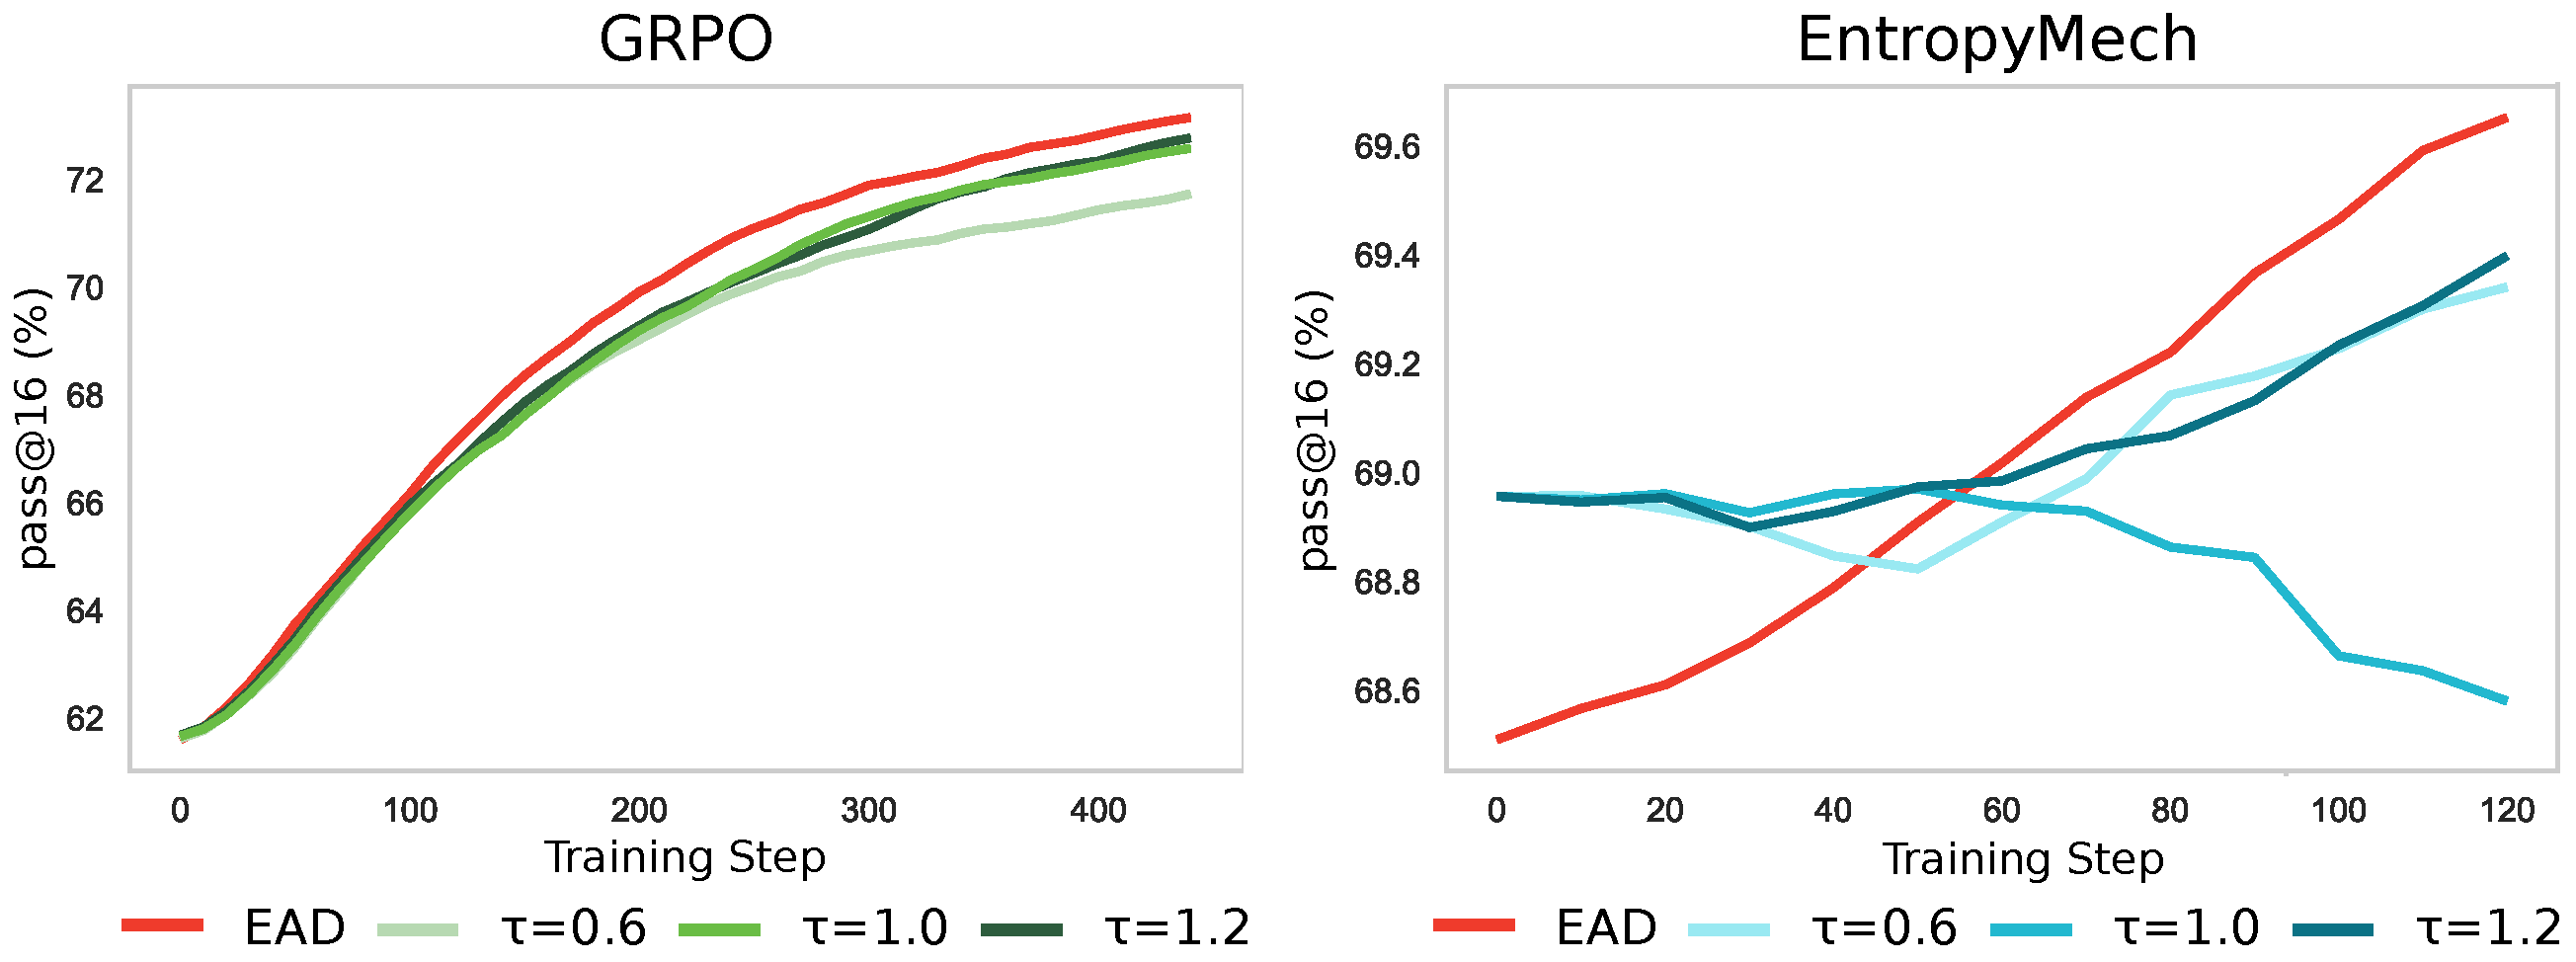
\includegraphics[width=0.98\linewidth]{figures/diff-method.pdf}
    \vspace{-5pt}
    \caption{
        \alg compatibility across RL algorithms. It consistently improves model performance over time compared to baselines.
    }
    \label{fig: algorithm_wide_comparison}
    \vspace{-10pt} % Adjust to minimize vertical space below the caption
\end{wrapfigure}
To demonstrate that \alg is a general, plug-and-play exploration strategy, we evaluate its performance when integrated into two other prominent RL algorithms: GRPO~\citep{shao2024deepseekmath} and EntropyMech~\citep{cui2025entropy}. 
%
These algorithms provide diverse testbeds. 
%
GRPO is more conservative, constraining policy updates with a KL divergence penalty and stricter clipping mechanism that can limit exploration~\citep{yu2025dapo}, while EntropyMech uses a specialized token-clipping mechanism to mitigate entropy collapse. 
%
As shown in \cref{fig: algorithm_wide_comparison}, \alg consistently outperforms fixed-temperature sampling in both frameworks. 
%
These results confirm the broad applicability of our method as an improved exploration strategy across different RL algorithms.
% \begin{wrapfigure}{r}{.5\linewidth}
%     \centering
%     % \vspace{-0.5in}
%     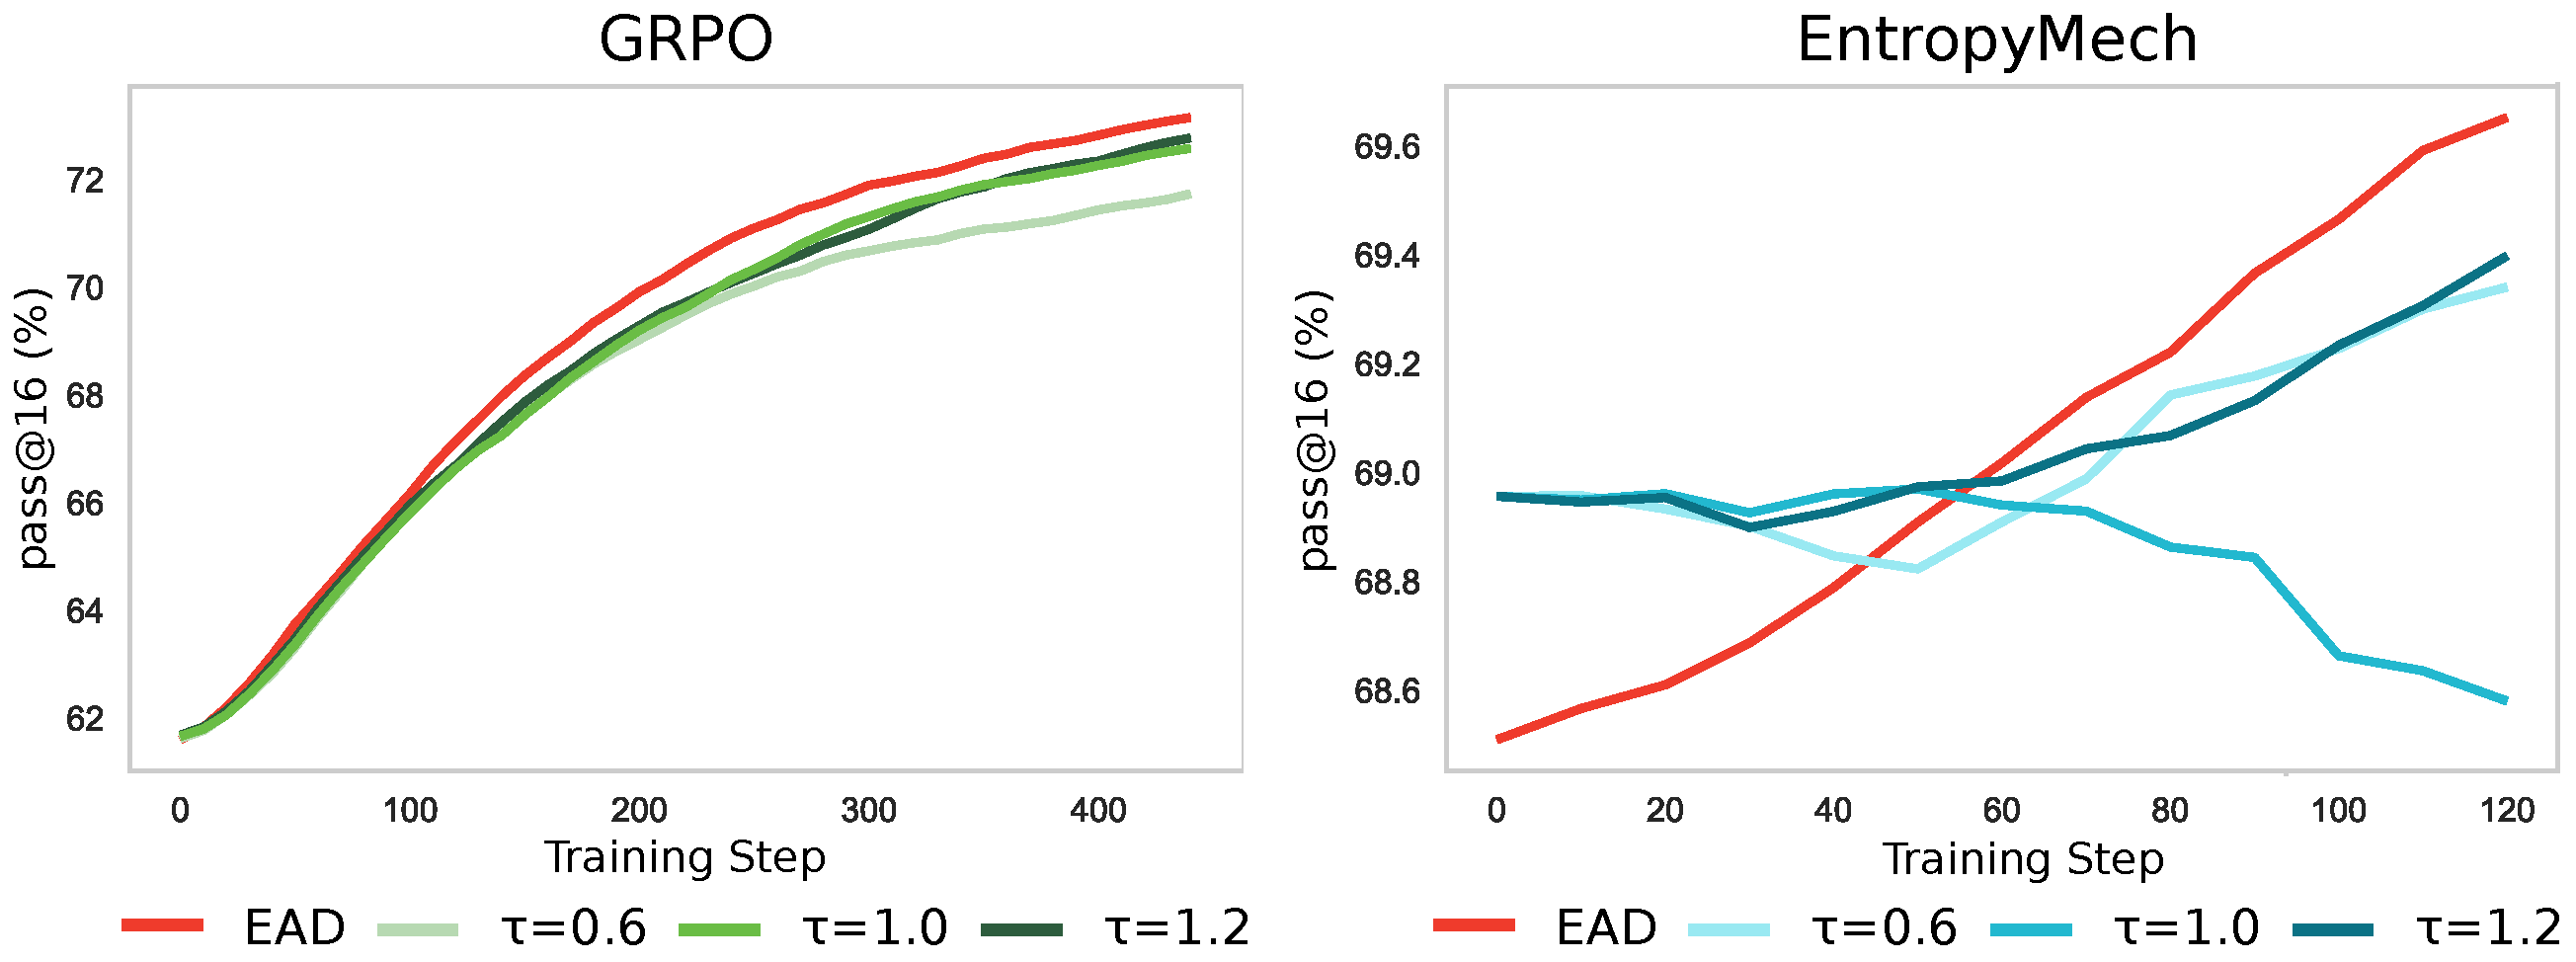
\includegraphics[width=\linewidth]{figures/diff-method.pdf}
%     \vspace{-0.1in}
%     \caption{\alg is compatible with various RL algorithms and can significantly improve the model performance over time. } 
%     \label{fig: algorithm_wide_comparison}
%     \vspace{-0.2in}
%     \end{wrapfigure}
%

\begin{figure}[t]
    \centering
\begin{subfigure}{0.48\linewidth}
    \centering
    % \vspace{-0.1in}
    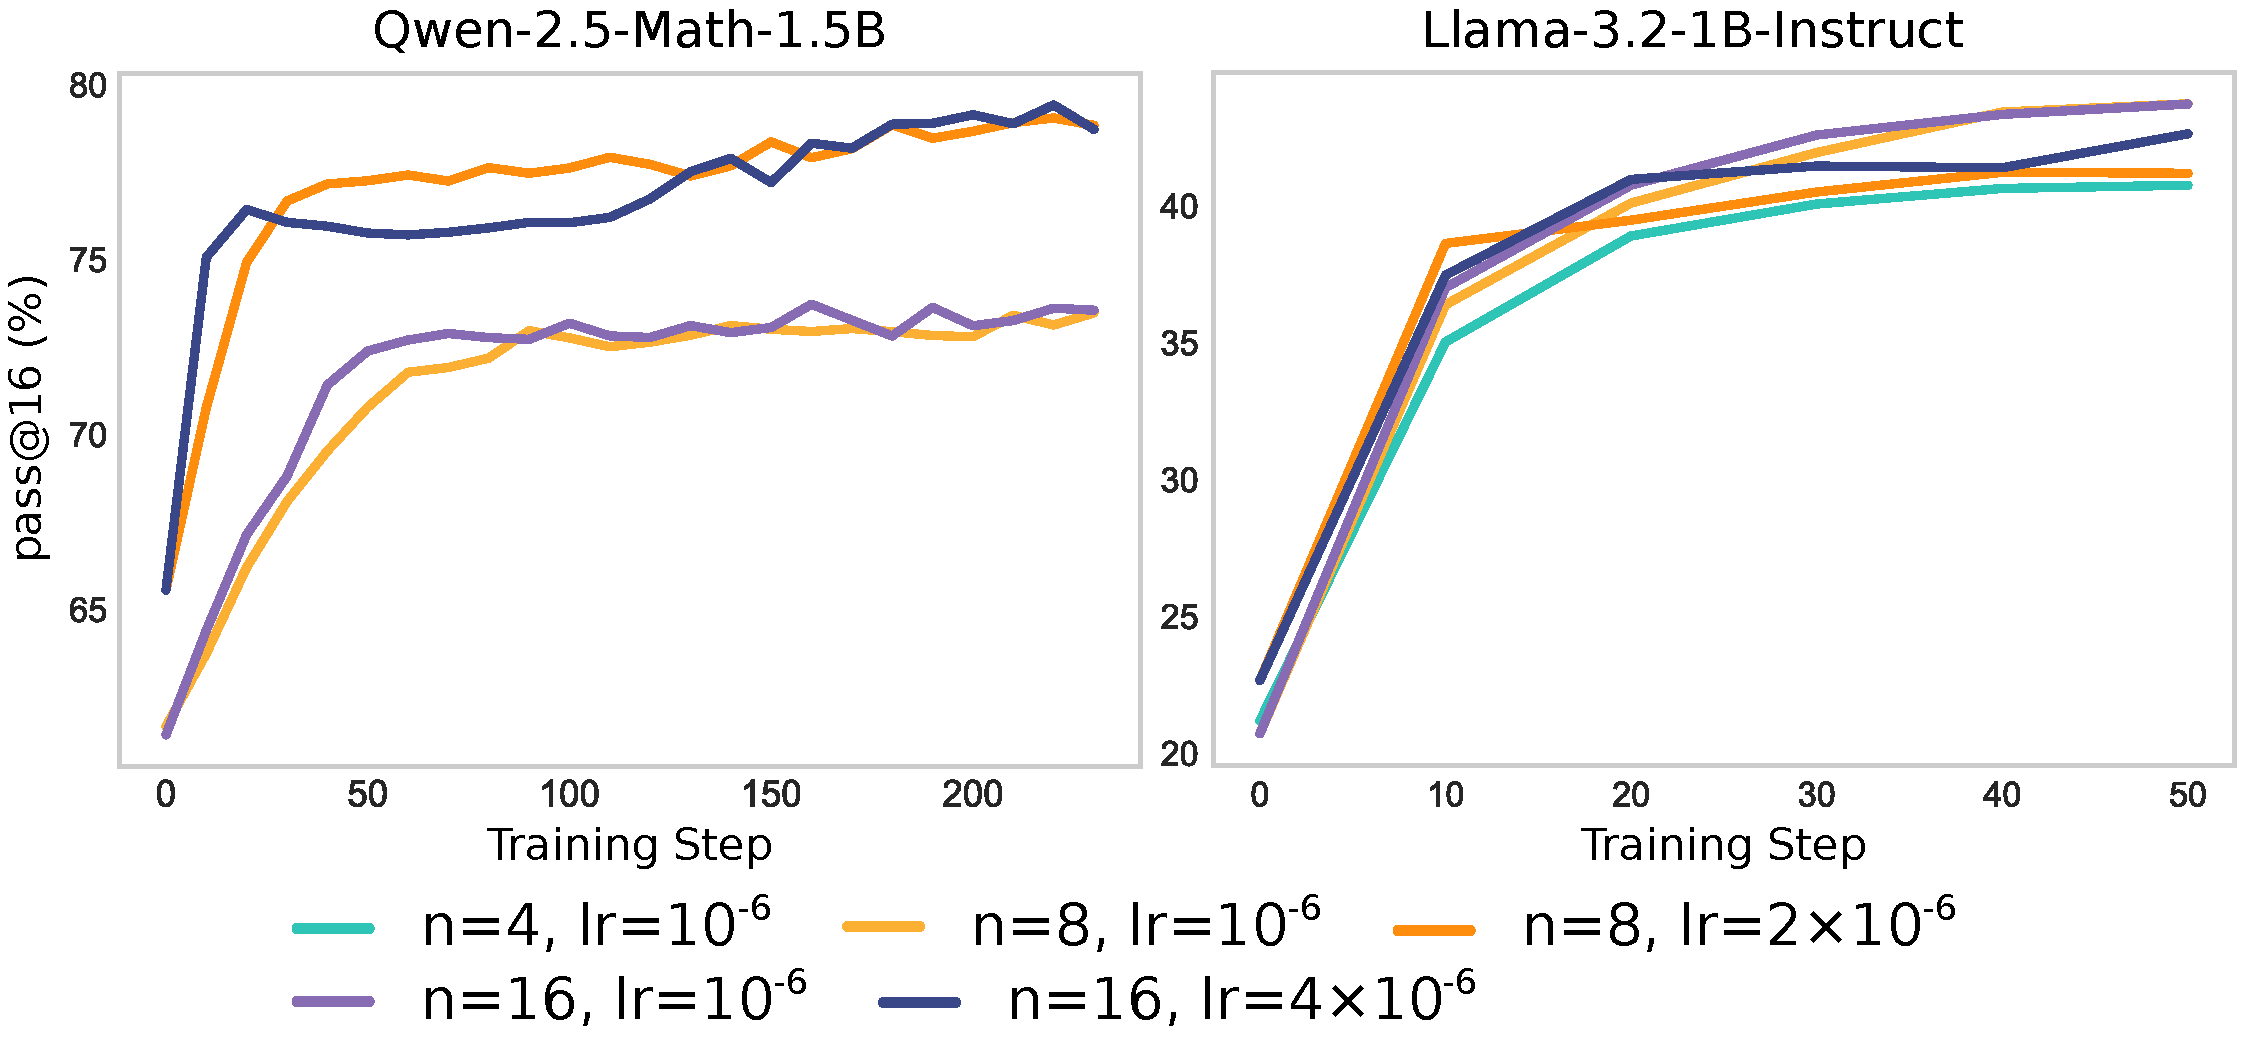
\includegraphics[width=\linewidth]{figures/scaling-rollout.pdf}
    % \vspace{-0.15in}
    \caption{\alg would bring further performance improvement via increased numbers of rollouts, but the commonly used $4$ / $8$ is already good enough. }
    \label{fig: main_bench_rollout_scaling}
% \vspace{-0.4in}
\end{subfigure}
% \end{figure}
\hfill
\begin{subfigure}{0.5\linewidth}
% \begin{figure}[h!]
    \centering
        % \vspace{-200pt}
    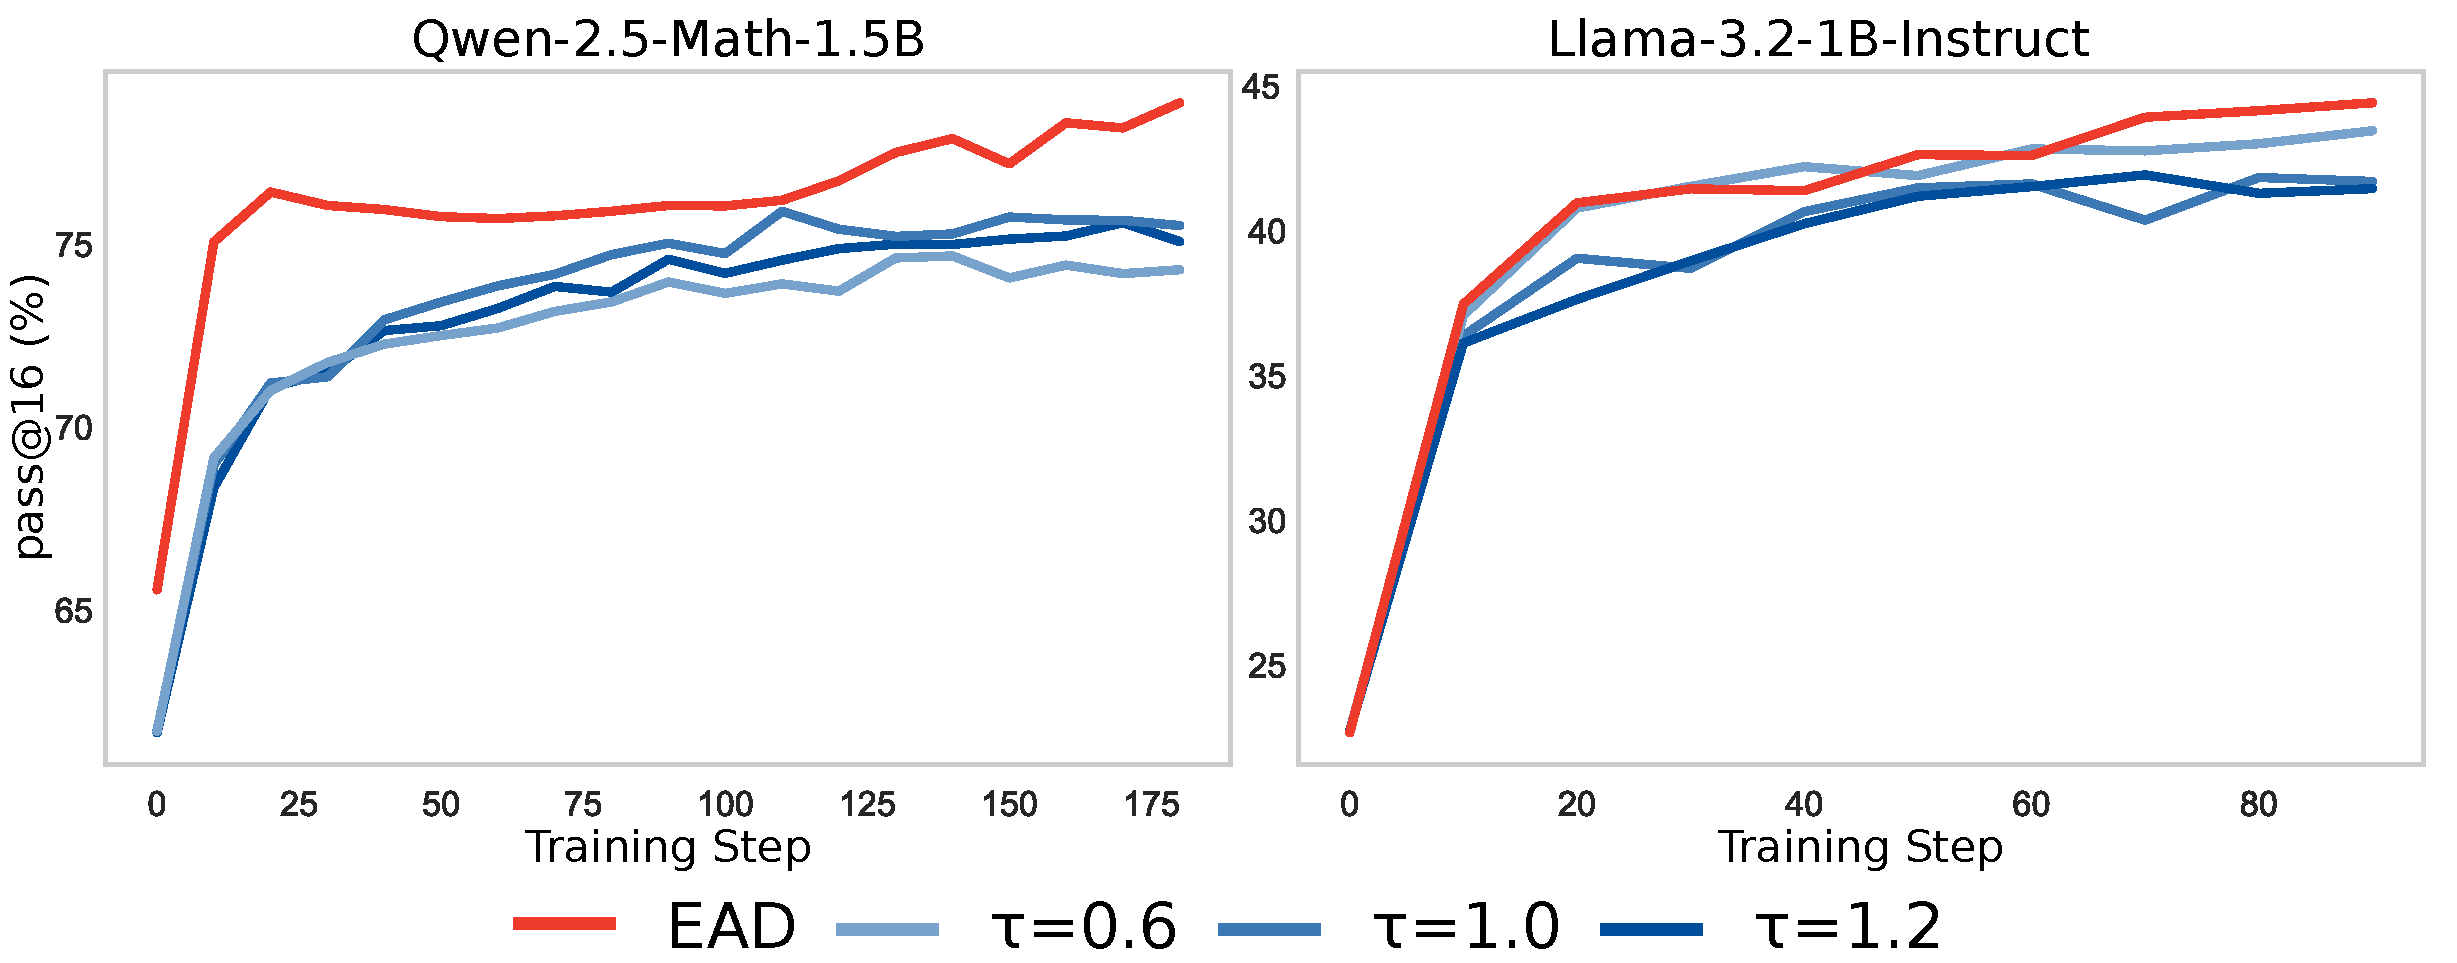
\includegraphics[width=0.99\linewidth]{figures/rollout-16-modelwise-compare.pdf}
    % \vspace{-0.25in}
    \caption{When scaling out the rollout number to 16, the relative advantages of \alg diminished; however, it still outperforms traditional same-temperature sampling.}
    \label{fig: rollout_modelwise_compare}
    % \vspace{-0.1in}
% \end{figure}
\end{subfigure}
\vspace{-5pt}
\caption{Impact of rollout numbers for \alg. }
\vspace{-25pt}
\end{figure}

\subsection{\alg Improves Inference-Time Scaling}
\begin{wrapfigure}{r}{0.5\textwidth}
    \centering
    % \vspace{-15pt} % Adjust to align top with the text
    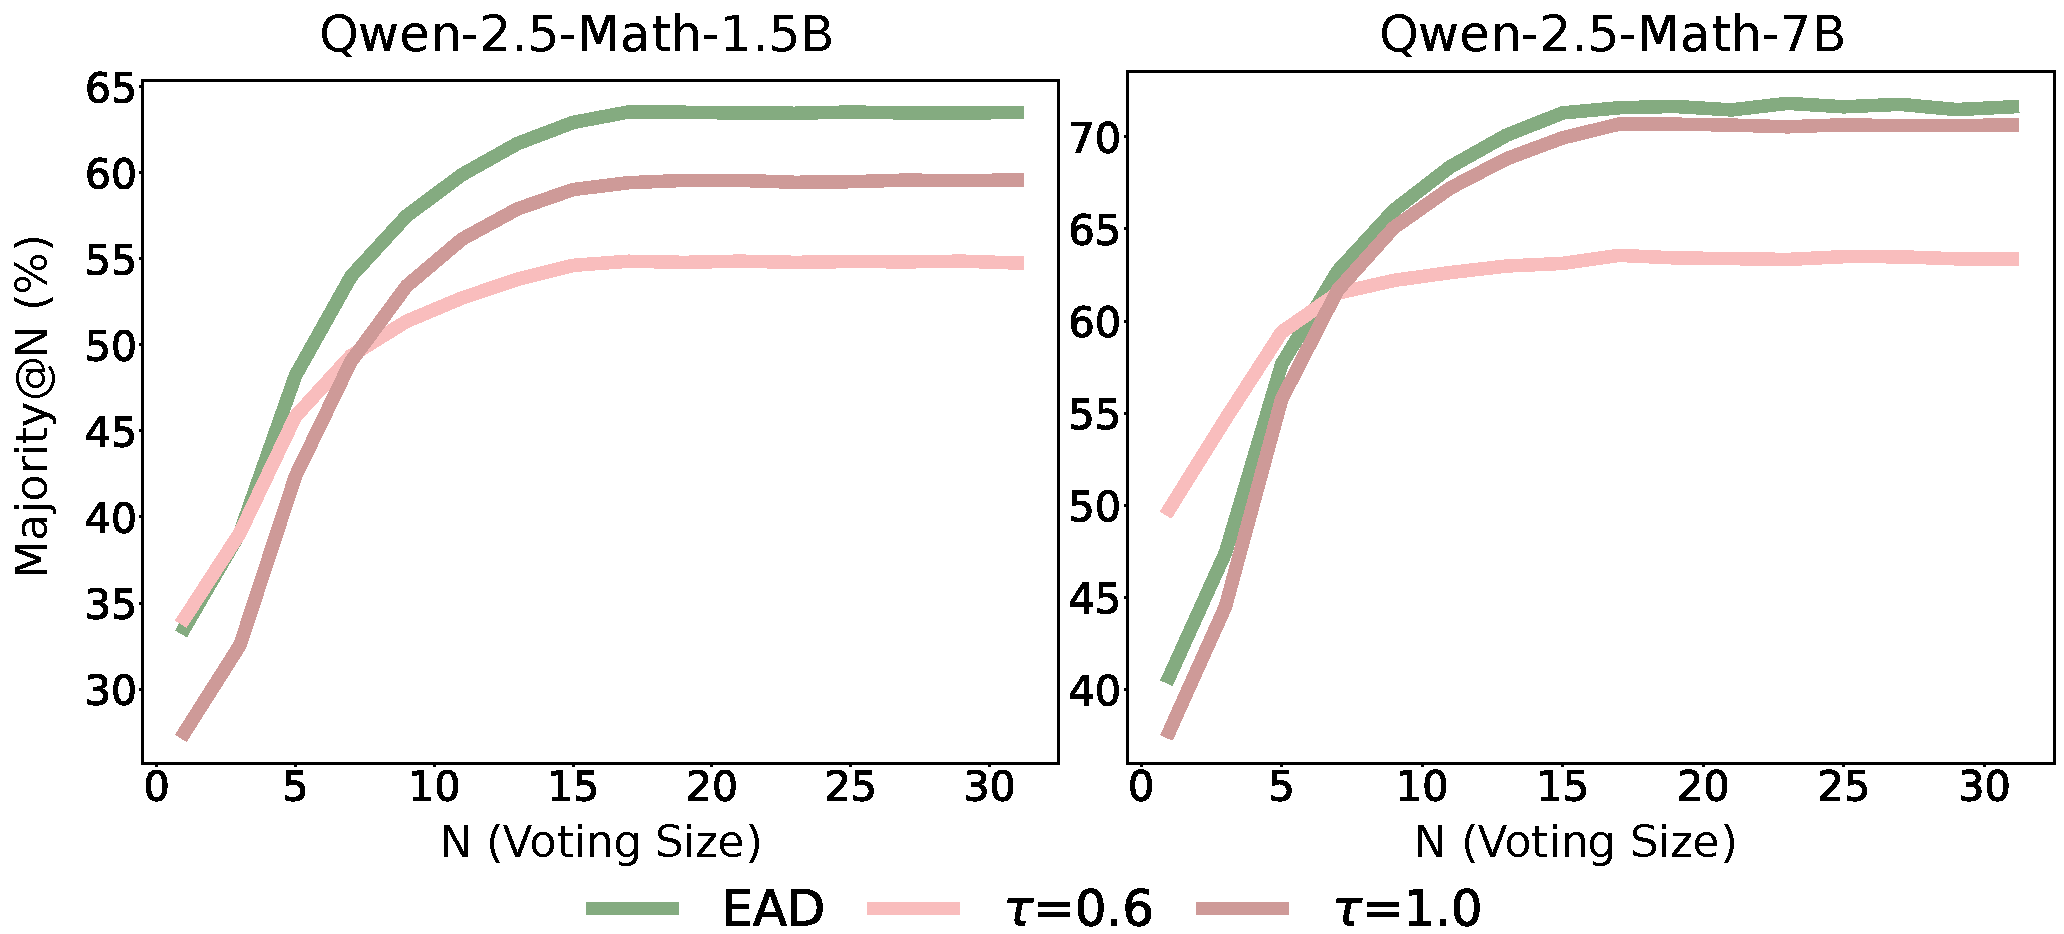
\includegraphics[width=\linewidth]{figures/inference-time-scaling.pdf}
    \vspace{-15pt}
    \caption{
        Inference-Time Scaling for Qwen2.5. \alg improves traditional sampling. Parameters: $\tau_{\text{max}}=1.2, \tau_{\text{min}}=0.1, d=25$.
    }
    \label{fig: inference_time_scaling}
    \vspace{-15pt} % Adjust to manage bottom spacing
\end{wrapfigure}


%
To understand whether the success of \alg in RL training is driven by its ability to generate high-quality samples, we conduct an evaluation at inference time. 
%
This experiment is designed to isolate the sampling strategy's effectiveness from the dynamics of RL optimization~\citep{berseth2025exploration}. 
%
Using off-the-shelf Qwen-2.5 models without any fine-tuning, we compare \alg against fixed-temperature sampling. 
%
Since no oracle is available at inference time to select the single correct answer from $N$ candidates, we adopt majority voting ($\text{Majority}@N$)~\citep{wang2023selfconsistency, snell2024scaling}, the standard practical aggregation strategy for inference-time scaling. 
%
As shown in \cref{fig: inference_time_scaling}, \alg consistently improves over the baseline for most values of $N$. 
%
% \begin{wrapfigure}{r}{.45\linewidth}
%     \centering
%     \vspace{-0.7in}
%     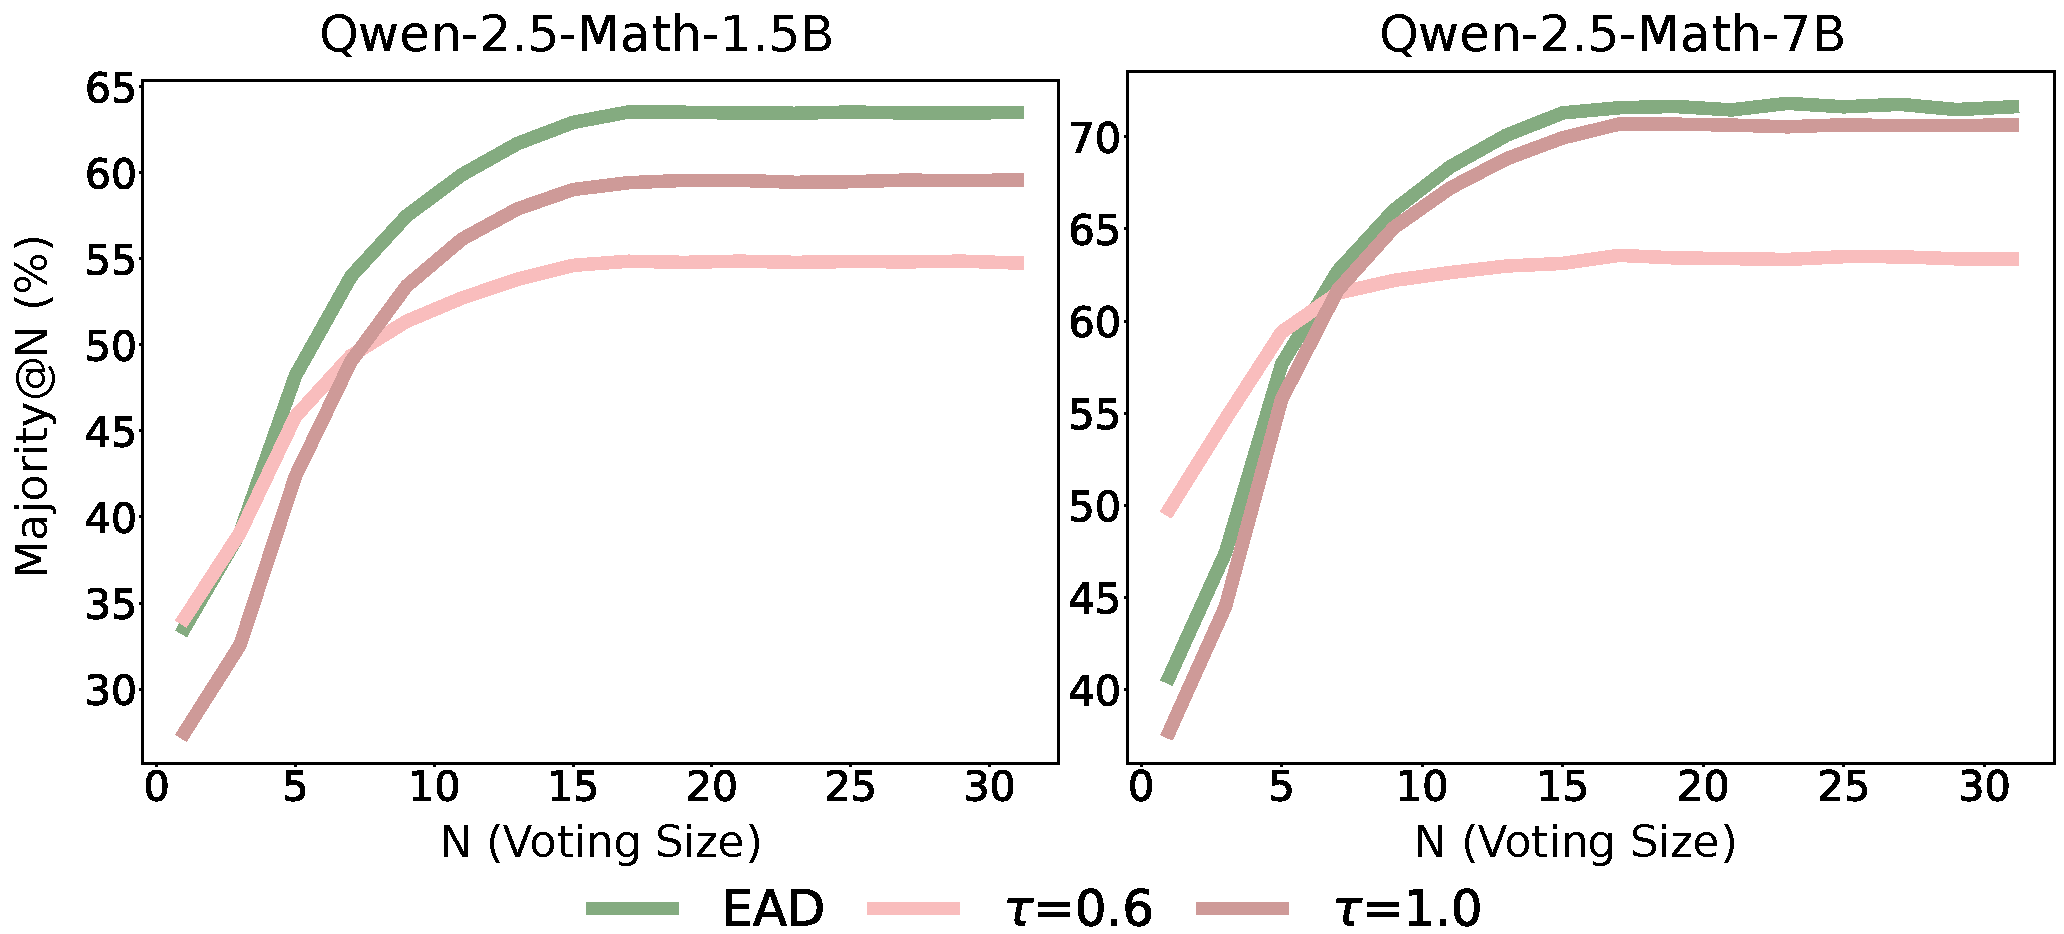
\includegraphics[width=\linewidth]{iclr2026/figures/inference_time_scaling/test-time.pdf}
%     % \vspace{-0.25in}
%     \caption{Inference-Time Scaling Evaluation for Different Decoding Methods using off-the-shelf Qwen2.5 models. We could see that \alg improves traditional temperature sampling. We set $\tau_{\text{max}}=1.2, \tau_{\text{min}}=0.1, d=25$ for \alg. }
%     \label{fig: inference_time_scaling}
%     \vspace{-0.2in}
%     \end{wrapfigure}
%
This result suggests that \alg's temperature schedule produces samples that are not only diverse but also of sufficiently high quality to improve the majority-voted consensus, even without any RL training.
%

\subsection{Ablation Study}
\label{sec:ablation_study}
\begin{wrapfigure}{r}{0.33\textwidth}
    \centering
    \vspace{-25pt} % Pull the figure up to align with the paragraph start
    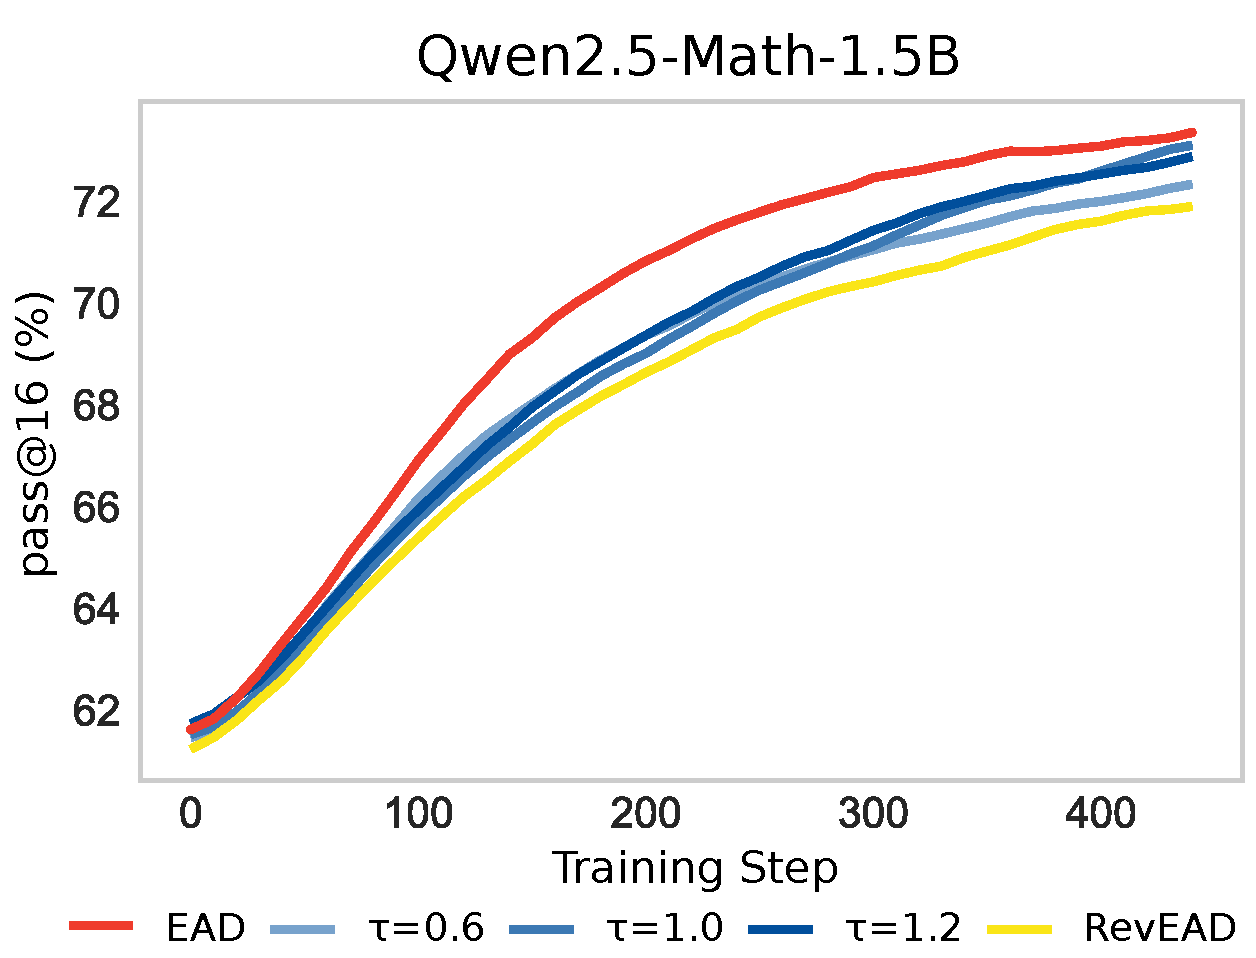
\includegraphics[width=\linewidth]{figures/reverse-annealing.pdf}
    \vspace{-20pt}
    \caption{
        Reverse Annealing results. A reverse schedule fails to surpass standard temperature sampling.
    }
    \label{fig: reverse_annealing}
    \vspace{-22pt} % Tighten the space below the caption
\end{wrapfigure}
\shortparagraph{Reverse Annealing.} We also test a reverse schedule, dubbed ``RevEAD'', where temperature increases during generation:
$\tau_t = \min\{\tau_\mathrm{min} + e^{t/d}, \tau_\mathrm{max}\}$.
As shown in \cref{fig: reverse_annealing}, RevEAD fails to even outperform standard temperature sampling, validating the necessity of an annealing (decreasing) temperature schedule. \revise{This observation also supports our hypothesis that late-stage exploration can be detrimental, potentially leading to high-variance ``lucky'' successes rather than robust reasoning paths.}

\shortparagraph{Hyperparameter Sensitivity, Scheduling Effects and Stress Test.}
We ablate key hyperparameters of \alg in \cref{app:ablation_details}. Our analysis reveals two findings. First, the \emph{intra-sequence} annealing schedule is the primary source of \alg's improvement: even with a fixed decay rate ($d_0 = d_{\max} = 25$, removing training-step adaptation), \alg still outperforms the best fixed-temperature baseline. Second, the \emph{global-step-aware} decay rate provides important complementary gains by keeping the schedule well-calibrated as response lengths grow during training; without it, performance eventually drops. Overall, \alg is robust across a wide range of decay cap $d_{\max}$ and growth factor $\alpha$ values (\cref{fig: ablation_cap,fig: ablation_growth_factor_and_decay_freq_init}). We further stress-test \alg on the challenging AIME 2024 benchmark using the DAPO recipe with Qwen-3-8B-Base~\citep{yang2025qwen3}, confirming consistent improvements over fixed-temperature sampling (\cref{app:stress_test}).

% ===== BEGIN COLM REBUTTAL EDIT: schedule-shape + d_max + code reasoning =====
\colmedit{%
\shortparagraph{Schedule shape vs. entropy budget.}
To check that the benefit is not merely from injecting additional entropy, we sweep three alternative schedules with the same $(\tau_{\max},\tau_{\min},d_0,\alpha,d_{\max})$ as \alg: a linear schedule, a two-stage step schedule, and a fixed-temperature ``mean-matched'' control whose temperature equals the time-average of \alg's curve (so the per-token entropy budget is matched). Results in \cref{app:schedule_shapes} (\cref{fig:schedule_shapes}) show that \alg's smooth exponential decay outperforms all three, indicating that the gains come from \emph{the shape of the schedule}, not just from a larger entropy budget.

\shortparagraph{Code-reasoning experiments.}
To check that \alg's benefits are not specific to mathematical reasoning, we additionally evaluate it on a code-reasoning RLVR setup with Qwen-2.5-Coder-1.5B-Instruct on the code subset of PRIME-RL's Eurus-2 dataset~\citep{cui2025process}, with held-out evaluation on LiveCodeBench (release\_v2)~\citep{jain2024livecodebench} and HumanEval+~\citep{liu2023evalplus}. The full recipe (no Docker / no sandbox service; we use the existing PRIME-RL subprocess execution path with SIGALRM timeouts) is provided in \cref{app:code_experiments}. \alg matches or exceeds the best fixed-temperature baseline on both benchmarks while showing the same entropy-collapse mitigation as in the math setting.
}
% ===== END COLM REBUTTAL EDIT =====